\subsection{Translating Typing Rules to Synthesis Rules}
In summary of \autoref{subsection:moti-representation}, \mainname extends typing rules for synthesis with the two design choices:
\begin{itemize} 
    \item When applying a rule, instead of pattern matching, \mainname introduces rule parameters as fresh variables and solves the constraints between variables via unification.
    \item Whenever an executable predicate requires the value of an unknown variable, \mainname acquires this value directly from the LM.
\end{itemize}
With these ideas, typing rules can be restated as formal synthesis rules in a mechanical way, which will be elaborated in \autoref{sec:meta}. Here we shall illustrate this process with the \textsc{T-App} rule as in \autoref{figure:s-app}.

To synthesize programs in $\stlc$, a synthesis judgment takes the form:
\[
\stlctype{\sketch{\Gamma}}{\sketch{p}}{\sketch{t}} \leadsto \sigma
\]
\begin{itemize}
\item \label{sketch-label}The left side is an incomplete typing judgment, where $\sketch{\Gamma}$, $\sketch{p}$, and $\sketch{t}$ represent a (possibly) incomplete context, program, and type, respectively. For example, $\sketch{t}$ can be an unknown variable $\sk{t}$, a partially known type $\tcode{bool} \rightarrow \sk{t}$, or a fully known type $\tcode{bool} \rightarrow \tcode{bool}$.
\item The right side is an assignment $\sigma$ to all unknown variables on the left side.
\end{itemize}

This judgment means that \textbf{the left-hand side typing judgment can be properly completed by the right-hand side assignment}; in other words, after applying $\sigma$ as a substitution, $\stlctype{\sigma(\sketch{\Gamma})}{\sigma(\sketch{p})}{\sigma(\sketch{t})}$ will be a valid typing judgment in the type system of $\stlc$. 
From the perspective of proof construction, the synthesis judgment corresponds to constructing an existential proof: given a proof goal with unknown variables, the synthesis process finds witnesses (i.e., concrete values for these variables) and proves the validity of the goal.  

\begin{figure*}
\centering 
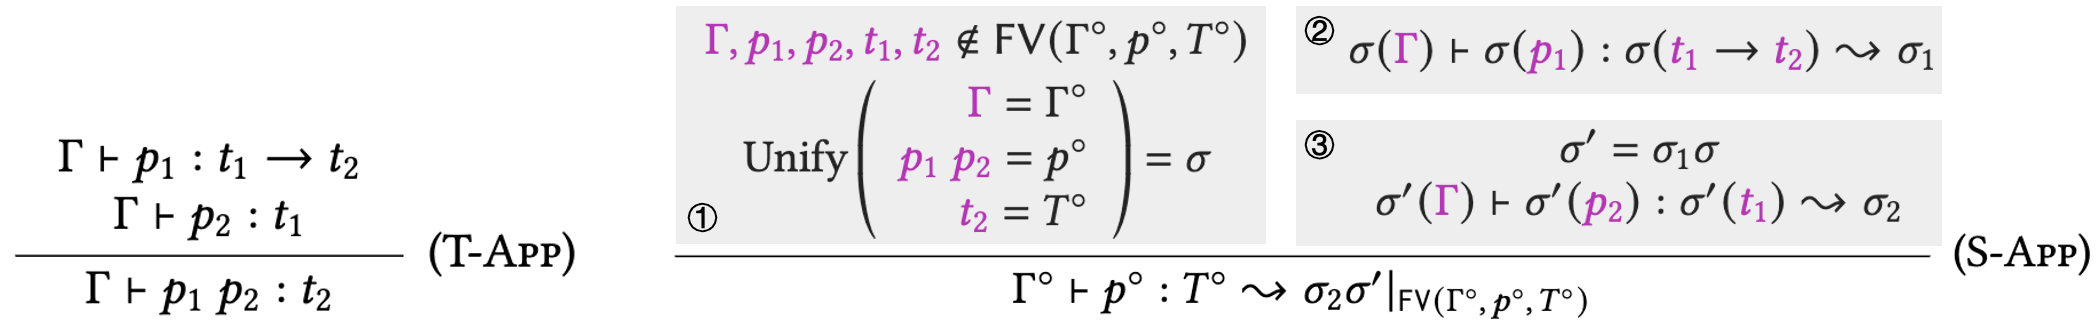
\includegraphics[width=\textwidth]{assets/S-App.png}
\caption{The typing rule \textsc{T-App} and its corresponding synthesis rule \textsc{S-App}, where $\textsf{FV}(\sketch{\Gamma}, \sketch{p}, \sketch{T})$ denotes the unknown variables in the incomplete typing judgment. \textsc{S-App} will return assignments only for these variables.} \label{figure:s-app}
\end{figure*}

As marked in \autoref{figure:s-app}, the premises of rule \textsc{S-App} can be divided into three parts.
\begin{itemize}
    \item Part 1 introduces a fresh variable for each parameter in the typing rule \textsc{T-App}, unifies the conclusion of \textsc{T-App} with the current incomplete typing judgment (i.e., $\stlctype{\sk{\Gamma}}{\sk{p_1}~\sk{p_2}}{\sk{t}}$ with $\stlctype{\sketch{\Gamma}}{\sketch{p}}{\sketch{t}}$) and thus extracts the relation between variables as a substitution $\sigma$.
    \item Parts 2 and 3 are introduced regarding the two premises in the \textsc{T-App} rule.
    %
    Part 2 completes the first premise $\stlctype{\Gamma}{p_1}{t_1 \rightarrow t_2}$, resulting in an assignment $\sigma_1$.
    %
    Then, Part 3 combines the known information by composing $\sigma$ and $\sigma_1$ into $\sigma'$, and further completes the second premise $\stlctype{\Gamma}{p_2}{t_1}$.
    %
    In general, this process repeats for all premises until each is completed, and any failure to discharge a premise causes the entire rule application to fail.
\end{itemize}

To get the result, \mainname composes the two obtained substitutions $\sigma_2$ and $\sigma'$.
Note that this composition involves not only variables in $\stlctype{\sketch{\Gamma}}{\sketch{p}}{\sketch{t}}$ but also local variables such as $\sk{\Gamma}$ and $\sk{p_1}$. 
Therefore, \textsc{S-App} will exclude these local variables and return only values of interest.

This translation establishes a direct correspondence between typing rules and synthesis rules. The core insight is that when the program is unknown, we can apply synthesis rules to construct an existential proof, which simultaneously discovers the program and proves its type correctness. The resulting existential proof has the same structure as the type correctness proof of the discovered program (like the one depicted in \autoref{figure:sample-type-tree}).

\endinput 
\noindent \textbf{Synthesis Rule for \textsc{T-Var}}. As a supplementary, \autoref{figure:s-var} shows the synthesis rule \textsc{S-Var}, extended from the \textsc{T-Var} rule.  
\newcommand{\remove}[1]{}
{
% 150\%
$$
\begin{prooftree}
    \hypo{\sk{\Gamma}, \sk{x}, \sk{t} \not \in \textsf{FV}(\sketch{\Gamma}, \sketch{p}, \sketch{T})}
    \infer[no rule]1{\quad\ \ \text{Unify}\left(
    \begin{array}{r}
        \sk{\Gamma}  =  \sketch{\Gamma} \\ 
        \sk{p_1~p_2}  = \sketch{p} \\ 
        \sk{t_2}  =  \sketch{T} 
    \end{array}
    \right) = \sigma\quad\ \ }
    \hypo{\stlctype{\sigma(\sk{\Gamma})}{\sigma(\sk{p_1})}{\sigma(\sk{t_1} \to \sk{t_2})} \leadsto \sigma_1}
    \infer[no rule]1{\sigma' = \sigma_1 \sigma}
    \infer[no rule]1{\ \ \stlctype{\sigma'(\sk{\Gamma})}{\sigma'(\sk{p_2})}{\sigma'(\sk{t_1})} \leadsto \sigma_2\ \ }
    \infer2[\textsc{(S-App)}]{\stlctype{\sketch{\Gamma}}{\sketch{p}}{\sketch{T}} \leadsto \sigma_2\sigma'|_{\mathtt{FV}(\sketch{\Gamma},\,\sketch{p},\,\sketch{T})}}
\end{prooftree}
$$
\vspace{1em}
$$
\begin{prooftree}
    \hypo{\checkBinding{\Gamma}{x}{t}}
    \infer1[\textsc{(T-Var)}]{\stlctype{\Gamma}{\vari x}{t}}
\end{prooftree}
$$
}

\remove{
% 150\%
$$
\begin{prooftree}
    \hypo{\sk{\Gamma, p_1, p_2, t_1, t_2} \not \in \textsf{FV}(\sketch{\Gamma}, \sketch{p}, \sketch{T})}
    \infer[no rule]1{\quad\ \ \text{Unify}\left(
    \begin{array}{r}
        \sk{\Gamma}  =  \sketch{\Gamma} \\ 
        \sk{p_1~p_2}  = \sketch{p} \\ 
        \sk{t_2}  =  \sketch{T} 
    \end{array}
    \right) = \sigma\quad\ \ }
    \hypo{\stlctype{\sigma(\sk{\Gamma})}{\sigma(\sk{p_1})}{\sigma(\sk{t_1} \to \sk{t_2})} \leadsto \sigma_1}
    \infer[no rule]1{\sigma' = \sigma_1 \sigma}
    \infer[no rule]1{\ \ \stlctype{\sigma'(\sk{\Gamma})}{\sigma'(\sk{p_2})}{\sigma'(\sk{t_1})} \leadsto \sigma_2\ \ }
    \infer2[\textsc{(S-App)}]{\stlctype{\sketch{\Gamma}}{\sketch{p}}{\sketch{T}} \leadsto \sigma_2\sigma'|_{\mathtt{FV}(\sketch{\Gamma},\,\sketch{p},\,\sketch{T})}}
\end{prooftree}
$$
\vspace{1em}
$$
\begin{prooftree}
    \hypo{\stlctype{\Gamma}{p_1}{t_1 \rightarrow t_2}}
    \infer[no rule]1{\qquad\stlctype{\Gamma}{p_2}{t_1}\qquad}
    \infer1[\textsc{(T-App)}]{\stlctype{\Gamma}{p_1~p_2}{t_2}}
\end{prooftree}
$$
}
